% \documentclass{ctexbeamer}
\documentclass{beamer}
\usepackage[scheme=plain]{ctex}
\usepackage{amsmath,amssymb}
\usepackage{amsthm}
% \usepackage{gbt7714}
\usepackage{subfig}
\usepackage{graphicx}
\usepackage{tikz}
% \usepackage[colorlink=true,xetex]{hyperref}

\usetheme{Madrid}
\usefonttheme[onlymath]{serif}
\bibliographystyle{IEEEtran}
\usetikzlibrary{graphs,quotes}
\usetikzlibrary{graphdrawing}
\usetikzlibrary{trees}
\usegdlibrary{trees}
\tikzset{
    rt/.style={draw=none,rectangle},
    normal/.style={draw,circle},
    cur/.style={fill=red!60},
    every picture/.style={}
}
\theoremstyle{plain}
% \newtheorem{theorem}{Theorem}
% \setbeamertemplate{background}{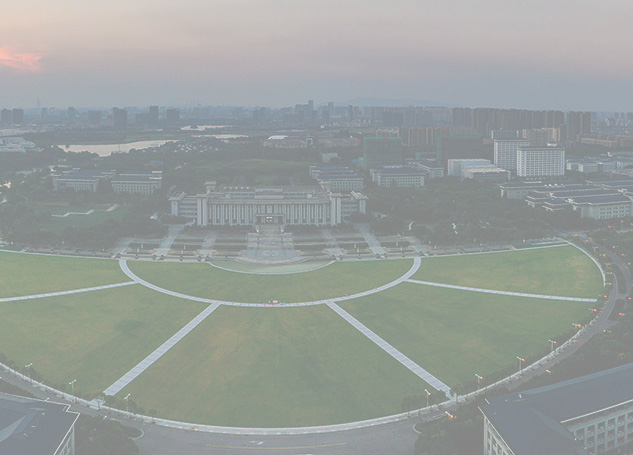
\includegraphics[height=\textwidth,clip]{pics/bg.jpg}}
% \usetikzlibrary{calc}

\title{Splay Tree and its Amortized Analysis}
\subtitle{A brief to Splay, the self-balanced binary search tree}
\input{personal_info/authors_fake.tex}

\begin{document}
    \begin{frame}
        \maketitle
    \end{frame}

    \begin{frame}
        \frametitle{Table of Contents}
    
        \tableofcontents
    
    \end{frame}

    \section{Introduction}

    \begin{frame}
        \frametitle{Inventors}
        \framesubtitle{Introduction}
    
        Splay trees were first introduced by Sleator and Tarjan in their article \textit{Self-adjusting binary search trees}, in 1985.

        \begin{figure}
            \centering
            \subfloat[Daniel Sleator]{
                \centering
                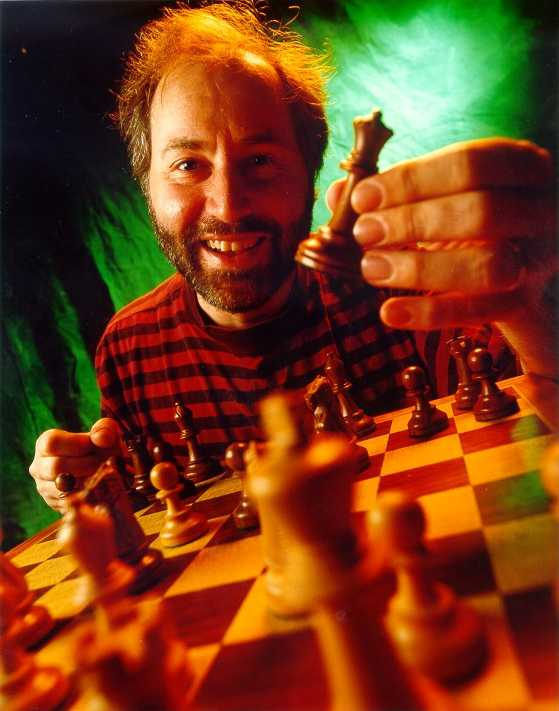
\includegraphics[height=0.45\textheight]{pics/Daniel_Sleator.jpg}
            }
            \qquad
            \subfloat[Robert Tarjan]{
                \centering
                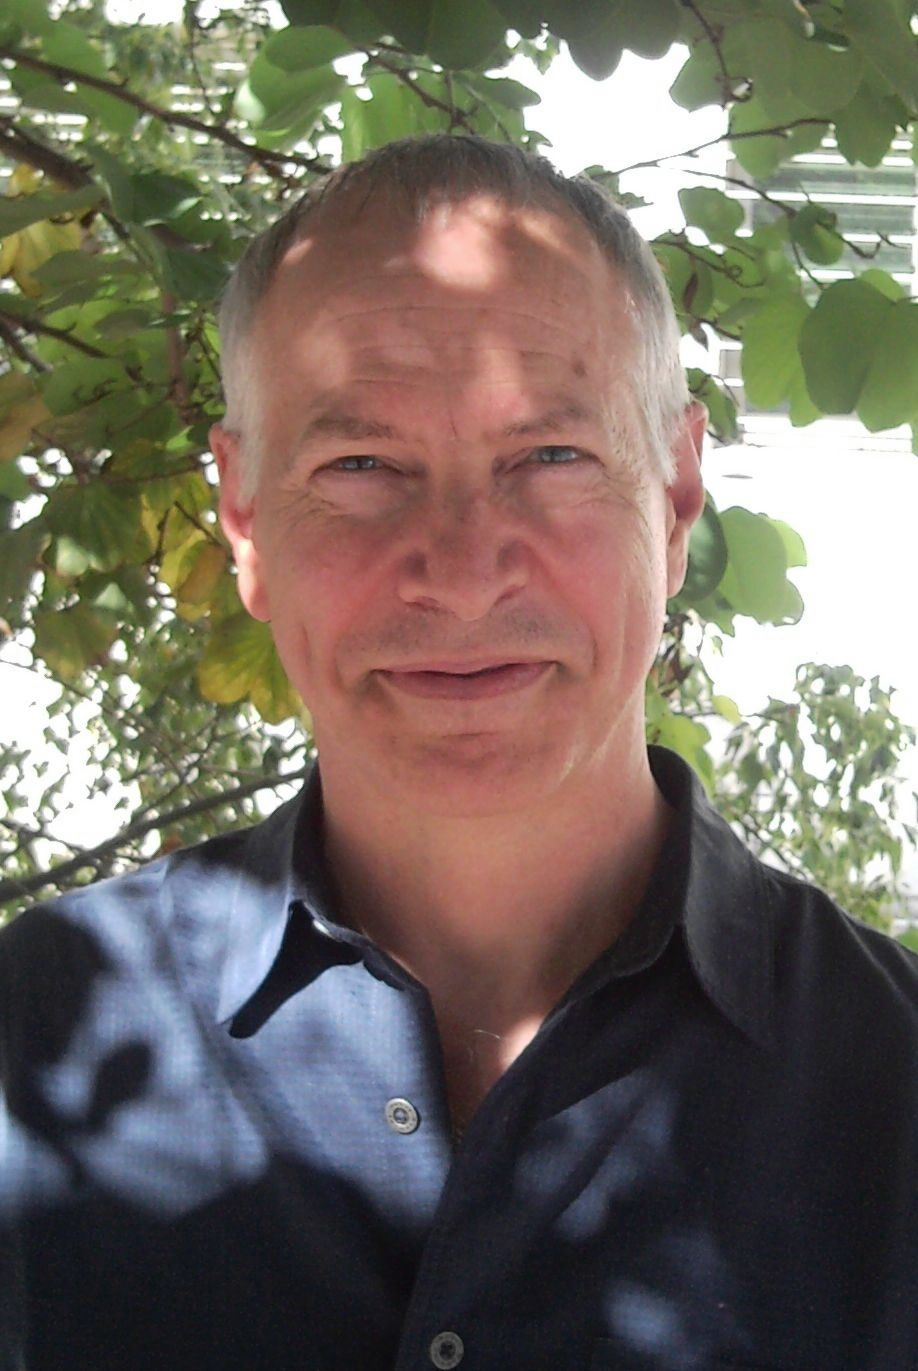
\includegraphics[height=0.45\textheight]{pics/Robert_Tarjan.jpg}
            }
            \caption{The inventors of Splay tree}
        \end{figure}
    
    \end{frame}

    \subsection{Motivation}

    \begin{frame}
        \frametitle{Motivation}
        \framesubtitle{Introduction}
    
        Efficient search trees have various drawbacks\cite{10.1145/3828.3835}:
        \begin{itemize}
            \item Not as efficient as possible if the access pattern is nonuniform;
            \item Need extra space for storage of balance information;
            \item Costs of insertion and deletion of optimum search trees are very high;
            \item Biased search trees are complicated in structure and hard to maintain;
            \item \textbf{Designed to reduce the worst-case time per operation}.
        \end{itemize}
    
    \end{frame}

    \section{Structure and Operations}
    \subsection{Structure of Splay Trees}

    \begin{frame}[fragile]
        \frametitle{Structure of Splay Trees}
    
        \begin{figure}
            \centering
            \subfloat[Fields of splay nodes]{
                \begin{tikzpicture}[nodes=normal]
                    \matrix (x) [rectangle,nodes={rectangle,text width=0.38\textwidth,align=center},label=Node $x$] {
                        \node (p) {Parent pointer ($p(x)$)}; \\
                        \node (l) {Left child pointer ($l(x)$)}; \\
                        \node (r) {Right child pointer ($r(x)$)}; \\
                        \node (val) {Item or item pointer ($v(x)$)}; \\
                    };
                \end{tikzpicture}
            }
            \quad
            \subfloat[Structure of splay tree]{
                \begin{tikzpicture}
                    \graph [binary tree layout,nodes=normal]{
                        "$root$"[rt] -> {,
                            a -- {
                                b -- {
                                    d, e
                                }, c -- {
                                    , f
                                }
                            }
                        }
                    };
                \end{tikzpicture}
            }
            \caption{Structure of Splay trees}
        \end{figure}

        \pause

        There is no additional fields that help keep the tree balanced, stored in splay nodes and splay trees.
    
    \end{frame}

    \subsection{Operations of Splay trees}

    \begin{frame}
        \frametitle{Overview}
        \framesubtitle{Operations of Splay trees}
    
        As BSTs, Splay trees have the normal operations as the other BSTs have:\pause

        \begin{itemize}
            \item $access(i, t)$: get the pointer to the node that stores the item $i$ from tree $t$, or $null$ if the node does not exist; \pause
            \item $insert(i, t)$: insert an item $i$ to the tree $t$, returing the pointer to the node contains it; \pause
            \item $remove(i, t)$: remove the node that stores item $i$ from tree $t$.
        \end{itemize}
    
    \end{frame}

    \begin{frame}
    
        To keep the implementations simple, there are two extra operations that should not be applied directly by the users: \pause

        \begin{itemize}
            \item $split(i, t)$: split the tree $t$ into 2 trees, $t_1$ and $t_2$, separately storing items the items that are not greater, and that are greater, than $i$; \pause
            \item $join(t_1, t_2)$: merge 2 trees $t_1$ and $t_2$ into a new tree $t$, returning the pointer to $t$'s root $rt(t)$. Every item in $t_1$ should be smaller than the items in $t_2$. \pause
        \end{itemize}

        And there is another operation that applied by the operations above, restructing the tree for optimization: \pause

        \begin{itemize}
            \item $splay(x)$: move a node $x$ to its tree's root, without destroying the BST.
        \end{itemize}
    
    \end{frame}

    \begin{frame}
        \frametitle{Access operation}
        \framesubtitle{Operations of Splay trees}
    
        Get the pointer to the node that stores a given item in the given tree.

        The only difference between Splay trees and other BSTs is that after the regular search operation, we apply the $splay$ operation to the node we visited latest.

        \begin{figure}
            \subfloat[Access the item]{
                \begin{tikzpicture}
                    \graph[binary tree layout,nodes=normal]{
                        "$root$"[rt] -> {,
                            42 -- {
                                18 -- {
                                    10, 35[cur]
                                },
                                60
                            }
                        }
                    };
                \end{tikzpicture}
            }
            \quad
            \subfloat[Splay the latest visited node]{
                \begin{tikzpicture}
                    \graph[binary tree layout,nodes={draw,circle}]{
                        "$root$"[rt] -> {,
                            35[cur] -- {
                                18 -- {
                                    10,
                                },
                                42 -- {
                                    , 60
                                }
                            }
                        }
                    };
                \end{tikzpicture}
            }
            \caption{Accessing an item that exists (35)}
        \end{figure}
    
    \end{frame}

    \begin{frame}[fragile]
    
        \begin{figure}
            \subfloat[Access the item]{
                \begin{tikzpicture}
                    \graph[binary tree layout,nodes=normal]{
                        "$root$"[rt] -> {,
                            42 -- {
                                18 -- {
                                    10, 35
                                },
                                60[fill=red!30] --[dashed] {
                                    null[dashed, cur],
                                }
                            }
                        }
                    };
                \end{tikzpicture}
            }
            \quad
            \subfloat[Splay the latest visited node]{
                \begin{tikzpicture}
                    \graph[binary tree layout,nodes={draw,circle}]{
                        "$root$"[rt] -> {,
                            60[fill=red!30] -- {
                                42 -- {
                                    18 -- {
                                        10, 35
                                    },
                                }
                            }
                        }
                    };
                \end{tikzpicture}
            }
            \caption{Accessing an non-exist item (50)}
        \end{figure}

        \pause

        Note that in the second situation, 60 was the latest visited node before we accessed $null$.
    
    \end{frame}

    \begin{frame}[fragile]
        \frametitle{Split operation}
        \framesubtitle{Operation of Splay trees}
    
        Access the given item $i$ first, then cut the edge links the new root and its left or right child.

        In the next example, we apply operation $split(50, t)$ and $split(35, t)$ separately.

        \begin{figure}
            \centering
            \subfloat[The original tree]{
                \begin{tikzpicture}
                    \graph[tree layout,nodes=normal]{
                        "$rt(t)$"[rt] -> {,
                            42 -- {
                                18 -- {
                                    10, 35
                                },
                                60 -- {
                                    , 75
                                }
                            }
                        }
                    };
                \end{tikzpicture}
            }
            \qquad
            \subfloat[Access the item]{
                \begin{tikzpicture}
                    \graph[tree layout,nodes=normal]{
                        "$rt(t)$"[rt] -> {
                            42 -- {
                                18 -- {
                                    10, 35
                                },
                                60[fill=red!30] -- {
                                    null[dashed, cur], 75
                                }
                            }
                        }
                    };
                \end{tikzpicture}
            }
            \caption{An example that cuts the left child}
        \end{figure}
    
    \end{frame}

    \begin{frame}
    
        \begin{figure}
            \subfloat[Splay the latest visited node]{
                \begin{tikzpicture}
                    \graph[tree layout,nodes={draw,circle}]{
                        "$rt(t)$"[rt] -> {,
                            60[fill=red!30] -- {
                                42 -- {
                                    18 -- {
                                        10, 35
                                    },
                                },
                                75
                            }
                        }
                    };
                \end{tikzpicture}
            }
            \quad
            \subfloat[Cut the edge]{
                \begin{tikzpicture}
                    \graph[tree layout, nodes=normal]{
                        "$rt(t_1)$"[rt] -> {
                            42 -- {
                                18 -- {
                                    10, 35
                                },
                            }
                        };
                        "$rt(t_2)$"[rt] -> {
                            60[fill=red!30] -- {
                                , 75
                            }
                        }
                    };
                \end{tikzpicture}
            }
            \caption{An example that cuts the left child (continued)}
        \end{figure}
    
    \end{frame}

    \begin{frame}[fragile]
        
        \begin{figure}
            \centering
            \subfloat[The original tree]{
                \begin{tikzpicture}
                    \graph[tree layout,nodes=normal]{
                        "$rt(t)$"[rt] -> {,
                            42 -- {
                                18 -- {
                                    10, 35
                                },
                                60 -- {
                                    , 75
                                }
                            }
                        }
                    };
                \end{tikzpicture}
            }
            \qquad
            \subfloat[Access the item]{
                \begin{tikzpicture}
                    \graph[tree layout,nodes=normal]{
                        "$rt(t)$"[rt] -> {,
                            35[cur] -- {
                                18 -- {
                                    10, 
                                },
                                42 -- {,
                                    60 --{,
                                        75
                                    }
                                }
                            }
                        }
                    };
                \end{tikzpicture}
            }
            \caption{An example that cuts the right child}
        \end{figure}
    
    \end{frame}

    \begin{frame}
    
        \begin{figure}
            \subfloat[Access the item]{
                \begin{tikzpicture}
                    \graph[tree layout,nodes=normal]{
                        "$rt(t)$"[rt] -> {,
                            35[cur] -- {
                                18 -- {
                                    10, 
                                },
                                42 -- {,
                                    60 --{,
                                        75
                                    }
                                }
                            }
                        }
                    };
                \end{tikzpicture}
            }
            \quad
            \subfloat[Cut the edge]{
                \begin{tikzpicture}
                    \graph[tree layout, nodes=normal]{
                        "$rt(t_1)$"[rt] -> {
                            35[cur] -- {
                                18 -- {
                                    10,
                                },
                            }
                        };
                        "$rt(t_2)$"[rt] -> {
                            42 -- {
                                , 60 -- {
                                    , 75
                                }
                            }
                        }
                    };
                \end{tikzpicture}
            }
            \caption{An example that cuts the right child (continued)}
        \end{figure}
    
    \end{frame}

    \begin{frame}
        \frametitle{Join operation}
        \framesubtitle{Operation of Splay trees}
    
        Apply $access(\max\{i \in t_1\}, t_1)$, or $access(+\infty, t_1)$, then set $rt(t_2)$ to the right child of $rt(t_1)$.
    
        \begin{figure}[fragile]
            \centering
            \subfloat[Initial status]{
                \begin{tikzpicture}
                    \graph[tree layout,nodes=normal]{
                        "$rt(t_1)$"[rt] -> {
                            20 -- {
                                , 40
                            }
                        };
                        "$rt(t_2)$"[rt] -> {
                            60 -- {
                                50, 80
                            }
                        }
                    };
                \end{tikzpicture}
            }
            \quad
            \subfloat[Access the maximum]{
                \begin{tikzpicture}
                    \graph[tree layout,nodes=normal]{
                        "$rt(t_1)$"[rt] -> {
                            40[cur] -- {
                                20,
                            }
                        };
                        "$rt(t_2)$"[rt] -> {
                            60 -- {
                                50, 80
                            }
                        }
                    };
                \end{tikzpicture}
            }
            \quad
            \subfloat[Connect the edge]{
                \begin{tikzpicture}
                    \graph[tree layout,nodes=normal]{
                        "$rt(t)$"[rt] -> {
                            40[cur] -- {
                                20, 60 -- {
                                    50, 80
                                }
                            }
                        }
                    };
                \end{tikzpicture}
            }
            \caption{Joining two trees}
        \end{figure}
    \end{frame}

    \begin{frame}[fragile]
        \frametitle{Insert operation}
        \framesubtitle{Operations of Splay trees}
    
        Assume that $i$ is not stored in tree $t$. \pause

        If $t$ is empty i.e. $rt(t) = null$, simply create a new node $x$ to store $i$, then set $rt(t) = x$. \pause

        Otherwise apply $split(i, t)$, getting two trees $t_1$ and $t_2$. Then create a new node $x$ to store $i$, and set $l(x) = rt(t_1), r(x) = rt(t_2), rt(t) = x$.

    \end{frame}

    \begin{frame}[fragile]
    
        \begin{figure}
            \centering
            \subfloat[The original tree]{
                \begin{tikzpicture}
                    \graph[tree layout,nodes=normal]{
                        "$rt(t)$"[rt] -> {,
                            42 -- {
                                18 -- {
                                    10, 35
                                },
                                60 -- {
                                    , 75
                                }
                            }
                        }
                    };
                \end{tikzpicture}
            }
            \quad\quad
            \subfloat[Apply the split]{
                \begin{tikzpicture}
                    \graph[tree layout, nodes=normal]{
                        "$rt(t_1)$"[rt] -> {
                            35 -- {
                                18 -- {
                                    10,
                                },
                            }
                        };
                        "$rt(t_2)$"[rt] -> {
                            42 -- {
                                , 60 -- {
                                    , 75
                                }
                            }
                        }
                    };
                \end{tikzpicture}
            }
            \caption{Inserting 40 to a non-empty tree}
        \end{figure}
    
    \end{frame}

    \begin{frame}[fragile]
    
        \begin{figure}
            \centering
            \subfloat[Create the new node]{
                \begin{tikzpicture}
                    \graph[tree layout, nodes=normal]{
                        "$rt(t_1)$"[rt] -> {
                            35 -- {
                                18 -- {
                                    10,
                                },
                            }
                        };
                        "$rt(t_2)$"[rt] -> {
                            42 -- {
                                , 60 -- {
                                    , 75
                                }
                            }
                        };
                        "$rt(t)$"[rt] -> {
                            40[cur]
                        }
                    };
                \end{tikzpicture}
            }
            \quad\quad
            \subfloat[Connect the edges]{
                \begin{tikzpicture}
                    \graph[tree layout, nodes=normal]{
                        "$rt(t)$"[rt] -> {
                            40[cur] -- {
                                35 -- {
                                    18 -- {
                                        10,
                                    },
                                },
                                42 -- {,
                                    60 -- {,
                                        , 75
                                    }
                                }
                            }
                        }
                    };
                \end{tikzpicture}
            }
            \caption{Inserting 40 to a non-empty tree (continued)}
        \end{figure}
    \end{frame}

    \begin{frame}[fragile]
        \frametitle{Remove operation}
        \framesubtitle{Operations of Splay trees}
    
        Assume that item $i$ exists in the tree $t$. \pause

        Apply $access(i, t)$, then cut the edges that connect $rt(t)$ with its childs. Finally apply $join$ to the two child trees.

        \begin{figure}
            \subfloat[Initial status]{
                \begin{tikzpicture}
                    \graph[tree layout, nodes=normal]{
                        "$rt(t)$"[rt] -> {
                            42 -- {
                                18 -- {
                                    10, 35
                                },
                                60
                            }
                        }
                    };
                \end{tikzpicture}
            }
            \quad
            \subfloat[Access the node]{
                \begin{tikzpicture}
                    \graph[tree layout, nodes=normal]{
                        "$rt(t)$"[rt] -> {
                            18[cur] -- {
                                10, 42 -- {
                                    35, 60
                                }
                            }
                        }
                    };
                \end{tikzpicture}
            }
            \quad
            \subfloat[Cut the edges]{
                \begin{tikzpicture}
                    \graph[tree layout, nodes=normal]{
                        "$rt(t_1)$"[rt] -> {
                            10
                        };
                        "$rt(t_2)$"[rt] -> {
                            42 -- {
                                35, 60
                            }
                        }
                    };
                \end{tikzpicture}
            }
            \caption{Removing 18 from a tree}
        \end{figure}
    
    \end{frame}

    \begin{frame}[fragile]
    
        \begin{figure}
            \subfloat[Apply the join operation]{
                \parbox{0.6\textwidth}{
                    \centering
                    \begin{tikzpicture}
                        \graph[tree layout, nodes=normal]{
                            "$rt(t)$"[rt] -> {
                                10 -- {,
                                    42 -- {
                                        35, 60
                                    }
                                }
                            }
                        };
                    \end{tikzpicture}
                }
            }
            \caption{Removing 18 from a tree (continued)}
        \end{figure}
    
    \end{frame}

    \begin{frame}[fragile]
        \frametitle{Rotation and Splaying}
        \framesubtitle{Operations of Splay trees}
    
        Splay operation is the key to keep the tree efficient. It consists of several splay steps, which are actually one or two rotations. \pause

        Rotation is an operation widely used in BST maintainance. There are 2 kinds of rotation: left-rotation and right-rotation.

        \begin{figure}
            \begin{tikzpicture}
                
                \scoped[nodes=normal] \node at (-2,0) {$z$}
                    child {node {$y$}
                        child {node {$x$}
                            child {node {$a$}}
                            child {node {$b$}}
                        }
                        child {node {$c$}}
                    }
                    child [missing];

                \scoped[nodes=normal] \node at (3,0) {$z$}
                    child {node {$x$}
                        child {node {$a$}}
                        child {node {$y$}
                            child {node {$b$}}
                            child {node {$c$}}
                        }
                    }
                    child [missing];

                \draw[->] (-1.25,-1.25) -- node[above] {right rotate $x$} ++(2.5,0);
                \draw[->] (1.25,-1.5) -- node[below] {left rotate $y$} ++(-2.5,0);
            \end{tikzpicture}
            \caption{Rotations}
        \end{figure}
    
    \end{frame}

    \begin{frame}
    
        Note that the direction of rotation is up to the relation between the node $x$ and its parent $p(x) = y$. So we can simply do $rotate(x)$ without telling its direction. \pause

        By applying $rotate$ operation once or twice, we get a $splay\ step$. It has 3 variants, depended on the relation between the node $x$, its parent $p(x)$ and its grandparent $g(x) = p(p(x))$.

        \begin{figure}
            \begin{tikzpicture}
                \scoped[nodes=normal] \node at (-3, 0) {$y$}
                    child {node {$x$}
                        child {node {$a$}}
                        child {node {$b$}}
                    }
                    child {node {$c$}};
                
                \scoped[nodes=normal] \node at (2, 0) {$x$}
                    child {node {$a$}}
                    child {node {$y$}
                        child {node {$b$}}
                        child {node {$c$}}
                    };
                
                    \draw[->] (-2, -1.25) -- node[above] {zig step} node[below] {$rotate(x)$} (1, -1.25);
            \end{tikzpicture}
            \caption{Variant 1: zig. Applied when $g(x) = null$.}
        \end{figure}
    
    \end{frame}

    \begin{frame}
    
        \begin{figure}
            \begin{tikzpicture}
                \scoped[nodes=normal] \node at (-4, 0) {$z$}
                    child {node {$y$}
                        child {node {$x$}
                            child {node {$a$}}
                            child {node {$b$}}
                        }
                        child {node {$c$}}
                    }
                    child {node {$d$}};

                \scoped[tree layout,nodes=normal] \node at (0, -1) {$y$}
                    child {node {$x$}
                        child {node {$a$}}
                        child {node {$b$}}
                    }
                    child {node {$z$}
                        child {node {$c$}}
                        child {node {$d$}}
                    };

                \scoped[nodes=normal] \node at (4, 0) {$x$}
                    child {node {$a$}}
                    child {node {$y$}
                        child {node {$b$}}
                        child {node {$z$}
                            child {node {$c$}}
                            child {node {$d$}}
                        }
                    };

                \draw[->] (-3, -1.25) -- node[above] {zig step} node[below] {$rotate(p(x))$} (-1.5, -1.25);
                \draw[->] (1.5, -1.25) -- node[above] {zig step} node[below] {$rotate(x)$} (3, -1.25);
            \end{tikzpicture}
            \caption{Variant 2: zig-zig. Applied when $x$ and $p(x)$ are in the same side of their parents.}
        \end{figure}
    
    \end{frame}

    \begin{frame}
    
        \begin{figure}
            \begin{tikzpicture}
                \scoped[nodes=normal] \node at (-4, 0) {$z$}
                    child {node {$y$}
                        child {node {$a$}}
                        child {node {$x$}
                            child {node {$b$}}
                            child {node {$c$}}
                        }
                    }
                    child {node {$d$}};

                \scoped[tree layout,nodes=normal] \node at (0, 0) {$z$}
                    child {node {$x$}
                        child {node {$y$}
                            child {node {$a$}}
                            child {node {$b$}}
                        }
                        child {node {$c$}}
                    }
                    child {node {$d$}};

                \scoped[level 1/.style={sibling distance=15mm},level 2/.style={sibling distance=8mm},nodes=normal] \node at (4, 0) {$x$}
                    child {node {$y$}
                        child {node {$a$}}
                        child {node {$b$}}
                    }
                    child {node {$z$}
                        child {node {$c$}}
                        child {node {$d$}}
                    };

                \draw[->] (-3, -1.25) -- node[above] {zig step} node[below] {$rotate(x)$} (-1.5, -1.25);
                \draw[->] (1, -1.25) -- node[above] {zag step} node[below] {$rotate(x)$} (2.5, -1.25);
            \end{tikzpicture}
            \caption{Variant 3: zig-zag. Applied when $x$ and $p(x)$ are not in the same side of their parents.}
        \end{figure}
    
    \end{frame}

    \begin{frame}
    
        For any given node $x$, we keep applying the different variants of $splay\ step$s on it, until $p(x) = null$ i.e. $x$ is the root of its tree. The continous operation is called $splay$, which also names the tree.
    
    \end{frame}

    \section{Amortized analysis}

    \begin{frame}
        \frametitle{Amortized analysis}
    
        Definitions:

        For any arbitary node $x$, or an arbitary tree $t$, we define that:

        \begin{itemize}
            \item $size, s(x)$: the size of the tree rooted at $x$, including $x$ itself; \pause
            \item $rank, r(x)$: $\log s(x)$, logarithm of $x$'s size; \pause
            \item $potential, \varPhi(t)$: sum of $r(x)$, where $x$ are all the nodes in the tree $t$.
        \end{itemize}

        Then we can prove that the amortized time $T_\mathrm{a}$ of a splay operation is at most: \[3(r(t) - r(x)) + 1 = O(\log \frac{s(t)}{s(x)})\]

        where $t$ is the root of the tree, and $x$ is the node to apply the operation.
    
    \end{frame}

    \begin{frame}[fragile]
        \frametitle{Zig step}
        \framesubtitle{Amortized analysis}
    
        Assume that $s'(x), r'(x)$ are $x$'s $size$ and $rank$ before applying the step:

        \begin{figure}
            \centering
            \begin{tikzpicture}
                \scoped[nodes=normal] \node [fill=green] at (-3, 0) {$y$}
                    child {node [fill=red!70] {$x$}
                        child {node {$a$}}
                        child {node {$b$}}
                    }
                    child {node {$c$}};
            
                \scoped[nodes=normal] \node [fill=red!70] at (2, 0) {$x$}
                    child {node {$a$}}
                    child {node [fill=green] {$y$}
                        child {node {$b$}}
                        child {node {$c$}}
                    };
            
                \draw[->] (-2, -1.25) -- node[above] {zig step} (1, -1.25);
            \end{tikzpicture}
        \end{figure}

        Total time $T_\mathrm{t1} = 1$, potential change $\Delta\varPhi = r(x) + r(y) - r'(x) - r'(y)$. So the amortized time is: \pause
        \begin{align*}
            T_\mathrm{a1} &= T_\mathrm{t1} + \Delta\varPhi = 1 + r(x) + r(y) - r'(x) - r'(y) \\
                         &\leq 1 + r(x) - r'(x) & \text{since } r(y) - r'(y) \leq 0 \\
                         &\leq 1 + 3(r(x) - r'(x)) & \text{since } r(x) - r'(x) \geq 0
        \end{align*}
    \end{frame}

    \begin{frame}
        \frametitle{Zig-zig steps}
        \framesubtitle{Amortized analysis}
    
        \begin{figure}
            \centering
            \begin{tikzpicture}
                \scoped[nodes=normal] \node [fill=green] at (-3, 0) {$z$}
                    child {node [fill=yellow] {$y$}
                        child {node [fill=red] {$x$}
                            child {node {$a$}}
                            child {node {$b$}}
                        }
                        child {node {$c$}}
                    }
                    child {node {$d$}};
            
                \scoped[nodes=normal] \node [fill=red!70] at (2, 0) {$x$}
                    child {node {$a$}}
                    child {node [fill=yellow] {$y$}
                        child {node {$b$}}
                        child {node [fill=green] {$z$}
                            child {node {$c$}}
                            child {node {$d$}}
                        }
                    };
            
                \draw[->] (-2, -1.5) -- node[above] {zig-zig step} (1, -1.5);
            \end{tikzpicture}
        \end{figure}
    
        Total time $T_\mathrm{t2} = 2$, potential change $\Delta\varPhi = r(x) + r(y) + r(z) - r'(x) - r'(y) -r'(z)$. So the amortized time is: \pause
        \begin{align*}
            T_\mathrm{a2} &= T_\mathrm{t2} + \Delta\varPhi
        \end{align*}
    \end{frame}

    \begin{frame}
    
        \begin{align*}
            &= 2 + r(x) + r(y) + r(z) - r'(x) - r'(y) - r'(z) \\
            &= 2 + r(y) + r(z) - r'(x) - r'(y) & \text{since } r(z) = r'(x) \\
            &\leq 2 + r(x) + r(z) - 2r'(x) & \text{since } r'(x) \leq r'(y) \\
            &                              & \text{and } r(x) \geq r(y)
        \end{align*}

        Since $\log x + \log y \leq -2$ when $x + y \leq 1, x,y > 0$, and $s'(x) + s(z) = s(x) - 1 \leq s(x)$, we get
        \begin{align*}
            2r(x) - r'(x) - r(z) = -(\log \frac{s'(x)}{s(x)} + \log \frac{s(z)}{s(x)}) \geq  2
        \end{align*}

        Then the amortized time is:
        \begin{align*}
            T_\mathrm{a2} \leq 3(r(x) - r'(x))
        \end{align*}
    
    \end{frame}

    
    \begin{frame}
        \frametitle{Zig-zag steps}
        \framesubtitle{Amortized analysis}
    
        \begin{figure}
            \centering
            \begin{tikzpicture}
                \scoped[nodes=normal] \node [fill=green] at (-3, 0) {$z$}
                    child {node [fill=green] {$y$}
                        child {node {$a$}}
                        child {node [fill=red] {$x$}
                            child {node {$b$}}
                            child {node {$c$}}
                        }
                    }
                    child {node {$c$}};
            
                \scoped[level 1/.style={sibling distance=15mm},level 2/.style={sibling distance=8mm},nodes=normal] \node [fill=red!70] at (2, 0) {$x$}
                    child {node [fill=green] {$y$}
                        child {node {$a$}}
                        child {node {$b$}}
                    }
                    child {node [fill=green] {$z$}
                        child {node {$c$}}
                        child {node {$d$}}
                    };
            
                \draw[->] (-2, -1.5) -- node[above] {zig-zag step} (0.5, -1.5);
            \end{tikzpicture}
        \end{figure}
    
        Total time $T_\mathrm{t3} = 2$, potential change $\Delta\varPhi = r(x) + r(y) + r(z) - r'(x) - r'(y) -r'(z)$. So the amortized time is: \pause
        \begin{align*}
            T_\mathrm{a3} &= T_\mathrm{t3} + \Delta\varPhi
        \end{align*}
    \end{frame}
    
    \begin{frame}
    
        \begin{align*}
            &= 2 + r(x) + r(y) + r(z) - r'(x) - r'(y) - r'(z) \\
            &= 2 + r(y) + r(z) - r'(x) - r'(y)  & \text{since } r'(z) = r(x) \\
            &\leq 2 + r(y) + r(z) - 2r'(x) & \text{since } r'(x) \leq r'(y)
        \end{align*}

        Since $\log x + \log y \leq -2$ when $x + y \leq 1, x,y > 0$, and $s(y) + s(z) = s(x) - 1 \leq s(x)$, we get
        \begin{align*}
            2r(x) - r(y) - r(z) = -(\log \frac{s(y)}{s(x)} + \log \frac{s(z)}{s(x)}) \geq  2
        \end{align*}

        Then the amortized time is:
        \begin{align*}
            T_\mathrm{a3} \leq 2(r(x) - r'(x)) \leq 3(r(x) - r'(x))
        \end{align*}
    
    \end{frame}

    \begin{frame}
        \frametitle{Theorem 1 (Balance Theorem)}
        \framesubtitle{Amortized analysis}
    
        Note that in a $splay$ operation we can apply at most 1 zig step. So by adding all $T_\mathrm{a}$ up, we get that the amortized time of a full $splay$ operation is:
        \[T_\mathrm{a} = 3(r(rt) - r(x)) + 1 = 3 \log \frac{n}{s(x)} + 1 \leq 3\log \frac{n}{1} + 1 = O(\log n)\]
        Where $n$ is the size of the whole tree. \pause

        After $m$ full $splay$ operations, the potential change is:
        \[\Delta\varPhi \geq \sum_{p \in \text{tree}} (0 - r(rt)) = \sum_{p \in \text{tree}} \log \frac{1}{n} = -n\log n\] \pause

        By using the formula $T_\mathrm{t} = T_\mathrm{a} - \Delta\varPhi$, we get the theorem:

        \begin{theorem}[Balance Theorem]
            The amortized time of $m$ full $splay$ operations is $T_\mathrm{t} = O((n + m)\log n + m)$.
        \end{theorem}
    
    \end{frame}

    \begin{frame}
        \frametitle{Other theorems}
    
        If we assign different positive weight $w(i)$ to each node in the tree, and redefine $s(n)$ as the sum of $w(i)$, then we get
        \[T_\mathrm{t} \leq 3(m \log \frac{W}{w(x)} + 1) + \sum_{p \in \text{tree}} \log \frac{W}{w(i)}\]
        Where $W = \sum_{p \in \text{tree}} w(p)$.

        By assigning proper value to $w(i)$, we can get even more theorems.
    
    \end{frame}

    \begin{frame}
    
        \begin{theorem}[Static Optimality Theorem]
            If every item is accessed at least once, the total time is \[T_\mathrm{t} \leq O(m + \sum_{i=1^n}q(i)\log \frac{m}{q(i)})\]
            Where $q(i)$ is the access frequency of item $i$.
        \end{theorem}

        \begin{theorem}[Static Finger Theorem]
            If $f$ is any fixed item, the total time is \[T_\mathrm{t} \leq O(n \log n + m + \sum_{j=1}^m \log (|i_j - f| + 1))\]
            Where $i_j$ is the $j$-th item in symmetric order.
        \end{theorem}

        % \begin{theorem}[Working Set Theorem]
        %     The total time is \[O(n \log n + m + \sum_{j=1}^m \log(t(j) + 1))\]
        %     Where $t(j)$ is the number of different items accessed before access $j$ since the last access of item $i_j$.
        % \end{theorem}
    
    \end{frame}

    \begin{frame}
        \frametitle{Conclusion}
        \framesubtitle{Amortized analysis}
    
        By redefining $potential\ \varPhi$, and using the same method above, we can conclude that, for any operation sequence, the total time
        is $O((n + m) \log n + m)$.
    
    \end{frame}

    \section{Applications}
    \begin{frame}
        \frametitle{Advantages and Disadvantages}
        \framesubtitle{Applications of Splay trees}
    
        Advantages: \pause
        \begin{enumerate}
            \item Easy to implement and maintain; \pause
            \item Require less space to store; \pause
            \item Can be much more efficient if usage pattern is skewed. \pause
        \end{enumerate}

        Disadvantages: \pause
        \begin{enumerate}
            \item Individual operations can be expensive.
        \end{enumerate}
    
    \end{frame}

    \begin{frame}
        \frametitle{GNU Projects}
        \framesubtitle{Applications of Splay trees}

        \begin{enumerate}
            \item GCC Compliers
            \item GOMP (GNU implementation of the OpenMP)
            \item libstdc++ (ext/pb\_ds)
        \end{enumerate}
    \end{frame}

    \begin{frame}
        \frametitle{Windows OS}
        \framesubtitle{Applications of Splay trees}
    
        Ntddk.h (Windows hardware driver and NTFS related)
    
    \end{frame}

    \begin{frame}
    
        \centering
        \huge Thanks for listening!
    
    \end{frame}

    \bibliography{citations}
\end{document}